\documentclass{article}
\usepackage[utf8x]{inputenc}
\usepackage{ucs}
\usepackage{amsmath} 
\usepackage{amsfonts}
\usepackage{marvosym}
\usepackage{wasysym}
\usepackage{upgreek}
\usepackage[english,russian]{babel}
\usepackage{graphicx}
\usepackage{float}
\usepackage{textcomp}
\usepackage{hyperref}
\usepackage{geometry}
  \geometry{left=2cm}
  \geometry{right=1.5cm}
  \geometry{top=1cm}
  \geometry{bottom=2cm}
\usepackage{tikz}
\usepackage{ccaption}
\usepackage{multicol}

\hypersetup{
   colorlinks=true,
   citecolor=blue,
   linkcolor=black,
   urlcolor=blue
}

\usepackage{listings}
%\setlength{\columnsep}{1.5cm}
%\setlength{\columnseprule}{0.2pt}

\usepackage[absolute]{textpos}

\usepackage{colortbl,graphicx,tikz}
\definecolor{X}{rgb}{.5,.5,.5}


\begin{document}
\pagenumbering{gobble}
\lstset{
  language=C,                % choose the language of the code
  basicstyle=\linespread{1.1}\ttfamily,
  columns=fixed,
  fontadjust=true,
  basewidth=0.5em,
  keywordstyle=\color{blue}\bfseries,
  commentstyle=\color{gray},
  stringstyle=\ttfamily\color{orange!50!black},
  showstringspaces=false,
  numbersep=5pt,
  numberstyle=\tiny\color{black},
  numberfirstline=true,
  stepnumber=1,                   % the step between two line-numbers.        
  numbersep=10pt,                  % how far the line-numbers are from the code
  backgroundcolor=\color{white},  % choose the background color. You must add \usepackage{color}
  showstringspaces=false,         % underline spaces within strings
  captionpos=b,                   % sets the caption-position to bottom
  breaklines=true,                % sets automatic line breaking
  breakatwhitespace=true,         % sets if automatic breaks should only happen at whitespace
  xleftmargin=.2in,
  extendedchars=\true,
  keepspaces = true,
  tabsize = 4,
}

\lstset{literate={~}{{\raisebox{0.5ex}{\texttildelow}}}{1}}
\newpage

\title{Семинар \#7: Память и бинарные файлы.\vspace{-5ex}}\date{}\maketitle

\section*{Системы счисления}
Мы привыкли пользоваться десятичной системой счисления и не задумываемся, что под числом в десятичной записи подразумевается следующее:
$$
123.45_{10} = 1 \cdot 10^2 + 2 \cdot 10^1 + 3 \cdot 10^0 + 4 \cdot 10^{-1} + 5 \cdot 10^{-2}
$$
Конечно, в числе 10 нет ничего сильно особенного с математической точки зрения. Оно было выбрано исторически, скорей всего по той причине, что у человека 10 пальцев. Компьютеры же работают с двоичными числами, потому что оказалось что процессоры на основе двоичной логики сделать проще. В двоичной системе счисления есть всего 2 цифры: \texttt{0} и \texttt{1}. Под записью числа в двоичной системе подразумевается примерно то же самое, что и в десятичной:
$$
101.01_2 = 1 \cdot 2^2 + 0 \cdot 2^1 + 1 \cdot 2^0 + 0 \cdot 2^{-1} + 1 \cdot 2^{-2} = 5.25_{10}
$$
При работе с компьютером на низком уровне имеет смысл использовать двоичную систему за место десятичной.  Но человеку очень сложно воспринимать числа в двоичной записи, так как они получаются слишком длинными. Поэтому популярность приобрели восьмеричная и шестнадцатиричная системы счисления. В шестнадцатиричной системе счисления есть 16 цифр: \texttt{0, 1, 2, 3, 4, 5, 6, 7, 8, 9, a, b, c, d, e, f}.
\begin{align*}
1a.8_{16} &= 1 \cdot 16^1 + 10 \cdot 16^0 + 8 \cdot 16^{-1} = 26.5\\
1ab_{16}  &= 1 \cdot 16^2 + 10 \cdot 16^1 + 11 = 427\\
ff.c_{16} &= 15 \cdot 16^ 1 + 15 \cdot 16^0 + 12 \cdot 16^{-1} = 255.75
\end{align*}

\subsection*{Шестнадцатиричная, восьмеричная и бинарная системы счисления в языке \texttt{C}}
Язык \texttt{C} поддерживает шестнадцатиричные, восьмеричные и бинарные литералы. Чтобы получить шестнадцатиричное число нужно написать \texttt{0x} перед числом. Чтобы получить восьмеричное число нужно написать \texttt{0} перед числом. Чтобы получить бинарное число нужно написать \texttt{0b} перед числом. 
\begin{lstlisting}
#include <stdio.h>
int main() 
{
    int a = 123;      // Десятичная система
    int b = 0x123;    // Шестнадцатиричная система
    int c = 0123;     // Восьмеричная система
    int d = 0b10101;  // Бинарная система
    printf("%i %i %i %i\n", a, b, c, d);
}
\end{lstlisting}
Также, можно печатать и считывать числа в других системах счисления с помощью спецификаторов \texttt{\%x} (для шестнадцатеричной -- he\textbf{x}adecimal) и \texttt{\%o} (для восьмеричной системы -- \textbf{o}ctal). Спецификатор \texttt{\%d} можно использовать для десятичной системы -- \textbf{d}ecimal (получается, что спецификатор \texttt{\%d} это то же самое, что и \texttt{\%i}). Для отображения адресов при печати с помощью спецификатора \texttt{\%p} используется шестнадцатеричная система счисления.
\begin{lstlisting}
#include <stdio.h>
int main() 
{
    int a;
    scanf("%d", &a);    // Считаем число в десятичной системе
    printf("%x\n", a);  // Напечатает это же число в шестнадцатеричной системе
    
    printf("%p\n", &a); // Для адресов используется шестнадцатеричная система
}
\end{lstlisting}


\section*{Представление чисел в памяти}

\subsection*{Представление целых чисел в памяти}
Положительные числа представляются в памяти в соответствии с их записью в бинарной системе счисления. Для представления отрицательных чисел в памяти используется способ, который называется дополнительный код. Однобайтовые числа представляются в памяти следующим образом:\\

\begin{minipage}{0.4\textwidth}
\begin{verbatim}
unsigned char
0        00000000
1        00000001
2        00000010
3        00000011
4        00000100
5        00000101
6        00000110
...
253      11111101
254      11111110
255      11111111
\end{verbatim}
\end{minipage}
\begin{minipage}{0.4\textwidth}
\begin{verbatim}
signed char
0        00000000
1        00000001
2        00000010
...
126      01111110
127      01111111
-128     10000000
-127     10000001
...
-2       11111110
-1       11111111
\end{verbatim}
\end{minipage}\\
\quad\\
\quad\\
Целые числа большего размера представляются в памяти аналогичным образом.
\subsection*{Представление чисел с плавающей точкой в памяти}
Разберём как числа с плавающей точкой хранятся в памяти на примере. Пусть у нас есть число $123.456$ типа \texttt{float}. Как это число хранится в двоичном коде? Для начала переведём это число из десятичной системы счисления в двоичную:
$$
123.456_{10} = 1111011.01110100101111000111_2
$$
Затем представим это число в научной записи:
$$
1111011.01110100101111000111_2 = 1.11101101110100101111000111_2 \cdot 2^6
$$
Получилось число:
\definecolor{c1}{RGB}{150,20,20}
\definecolor{c2}{RGB}{20,20,150}
\definecolor{c3}{RGB}{20,150,20}
$$
\color{c1}+\color{black}1.\color{c2}11101101110100101111000111\color{black}_2 \cdot 2^{\color{c3}6}
$$
Части этой записи числа и хранятся в памяти.
Число типа \texttt{float} имеет размер 4 байта или 32 бита. Из них:
\begin{itemize}
\item \color{c1}1 бит\color{black}\quad приходится на знак числа. 0 -- для положительных и 1 для отрицательных.
\item \color{c3}8 бит\color{black}\quad приходится на степень двойки. К степени двойки в двоичной научной записи прибавляется число 127, а затем это число хранится в этих битах.
В нашем примере будет храниться число $6 + 127 = 133 = 10000101_2$.
\item \color{c2}23 бита\color{black}\quad приходится на мантиссу. В двоичной научной записи это просто 23 цифры после точки. В нашем примере это $11101101110100101111001$ (округляем последнюю цифру).
\end{itemize}
Таким образом число $123.456$ типа \texttt{float} будет хранится в памяти как:
$$
0\ \ \ 10000101\ \ \ 11101101110100101111001
$$
Разобъем эту запись на кусочки по 8 бит:
$$
01000010\ \ \ 11110110\ \ \ 11101001\ \ \ 01111001
$$
Переведём каждый из кусочков в шестнадцатеричную систему:
$$
42\ \ \ F6\ \ \ E9\ \ \ 79
$$
Это значения которые будут иметь байты числа типа \texttt{float} при записи в него числа $123.456$.
Числа типа \texttt{double} хранятся аналогичным образом, но для хранения степени и мантиссы используется 11 и 52 бита соответственно.

\newpage
\subsection*{Побитовые операторы}


\subsubsection*{Побитовое И}
Побитовое И применяет операцию логического И для каждого бита. Обозначается символом \texttt{\&}.\\

\begin{minipage}{0.35\textwidth}
\begin{verbatim}
x     = 00010100 = 20
y     = 01100100 = 100
x & y = 00000100 = 4
\end{verbatim}
\end{minipage}
\hfill
\begin{minipage}{0.55\textwidth}
\begin{lstlisting}
printf("%i\n", 20 & 100);  // Напечатает 4
\end{lstlisting}
\end{minipage}

\subsubsection*{Побитовое ИЛИ}
Побитовое ИЛИ применяет операцию логического ИЛИ для каждого бита. Обозначается символом \texttt{|}.\\

\begin{minipage}{0.35\textwidth}
\begin{verbatim}
x     = 00010100 = 20
y     = 01100100 = 100
x | y = 01110100 = 116
\end{verbatim}
\end{minipage}
\hfill
\begin{minipage}{0.55\textwidth}
\begin{lstlisting}
printf("%i\n", 20 | 100);  // Напечатает 116
\end{lstlisting}
\end{minipage}
\subsubsection*{Побитовое исключающее ИЛИ}
Побитовое исключающее ИЛИ применяет операцию логического исключающее ИЛИ (также известную как \textit{exclusive OR} или просто \textit{XOR}) для каждого бита.  Операция логического исключающего ИЛИ задаётся следующими выражениями:
\begin{center}
\texttt{0 XOR 0 = 0}\\
\texttt{0 XOR 1 = 1}\\
\texttt{1 XOR 0 = 1}\\
\texttt{1 XOR 1 = 0}\\
\end{center}
Побитовое исключающее ИЛИ в коде обозначается символом \textsuperscript{$\wedge$}.\\

\begin{minipage}{0.35\textwidth}
\begin{verbatim}
x     = 00010100 = 20
y     = 01100100 = 100
x ^ y = 01110000 = 112
\end{verbatim}
\end{minipage}
\hfill
\begin{minipage}{0.55\textwidth}
\begin{lstlisting}
printf("%i\n", 20 ^ 100);  // Напечатает 112
\end{lstlisting}
\end{minipage}
\subsubsection*{Побитовое НЕ}
Побитовое НЕ применяет операцию логического НЕ для каждого бита. То есть просто обращает каждый бит числа. Обозначается символом $\sim$.\\

\begin{minipage}{0.35\textwidth}
\begin{verbatim}
x     = 00010100 = 20
~x    = 11101011 = -21
\end{verbatim}
\end{minipage}
\hfill
\begin{minipage}{0.55\textwidth}
\begin{lstlisting}
printf("%i\n", ~20);  // Напечатает -21
\end{lstlisting}
\end{minipage}

\subsubsection*{Побитовый сдвиг влево}
Побитовый сдвиг влево сдвигает все биты числа влево на заданное число. Обозначается как \texttt{<{}<}.\\

\begin{minipage}{0.35\textwidth}
\begin{verbatim}
x         = 00010100 = 20
x << 2    = 01010000 = 80
\end{verbatim}
\end{minipage}
\hfill
\begin{minipage}{0.55\textwidth}
\begin{lstlisting}
printf("%i\n", 20 << 2);  // Напечатает 80
\end{lstlisting}
\end{minipage}
\subsubsection*{Побитовый сдвиг вправо}
Побитовый сдвиг вправо сдвигает все биты числа вправо на заданное число. Обозначается как \texttt{>{}>}.\\

\begin{minipage}{0.35\textwidth}
\begin{verbatim}
x         = 00010100 = 20
x >> 2    = 00000101 = 5
\end{verbatim}
\end{minipage}
\hfill
\begin{minipage}{0.55\textwidth}
\begin{lstlisting}
printf("%i\n", 20 >> 2);  // Напечатает 5
\end{lstlisting}
\end{minipage}\\
\quad
\quad\\
Если побитовый сдвиг вправо применяется к отрицательному числу, то, на большинстве системах, левые биты заполняются не нулями а единицами:\\

\begin{minipage}{0.35\textwidth}
\begin{verbatim}
x         = 11101011 = -21
x >> 2    = 11111010 = -6
\end{verbatim}
\end{minipage}
\hfill
\begin{minipage}{0.55\textwidth}
\begin{lstlisting}
printf("%i\n", -21 >> 2);  // Напечатает -6
\end{lstlisting}
\end{minipage}
\quad\\
\quad\\
Если правый операнд операторов сдвига -- отрицательное число, то это UB.

\subsubsection*{Печать битового представления числа}
Данная функция печатает все биты числа типа \texttt{int}:
\begin{lstlisting}
#include <stdio.h>
void print_binary(const char* prefix, int x)
{
    printf("%s", prefix);
    for (int i = 8 * sizeof(x) - 1; i >= 0; --i)
    {
        printf("%u", (x >> i) & 1);
        if (i % 8 == 0)
            printf(" ");
    }
    printf("\n");
}
int main() 
{
    int x = 0b00010100;
    int y = 0b01100100;
    print_binary("x      = ", x);
    print_binary("y      = ", y);
    print_binary("x & y  = ", x & y);
    print_binary("x | y  = ", x | y);
    print_binary("x ^ y  = ", x ^ y);
    print_binary("~x     = ", ~x);
    print_binary("x << 2 = ", x << 2);
    print_binary("x >> 2 = ", x >> 2);
}
\end{lstlisting}

\subsubsection*{Получение значения \texttt{i}-го бита числа}
Для получения \texttt{i}-го бита числа (нумерировать биты будем, начиная с нуля) нужно сдвинуть число на \texttt{i} бит вправо и применить побитовое и с единицей.

\begin{minipage}{0.35\textwidth}
\begin{lstlisting}
x            = 00010100
x >> 2       = 00000101
(x >> 2) & 1 = 00000001
\end{lstlisting}
\end{minipage}
\hfill
\begin{minipage}{0.55\textwidth}
\begin{lstlisting}
int x = 0b00010100;
printf("%i\n", (x >> 2) & 1);
\end{lstlisting}
\end{minipage}


\subsubsection*{Установка \texttt{i}-го бита в значение \texttt{1}}
Для того, чтобы установить \texttt{i}-й бит числа в значение \texttt{1} нужно применить побитовое или с числом \texttt{(1 <{}< i)}.

\begin{minipage}{0.35\textwidth}
\begin{lstlisting}
x            = 00010100
1            = 00000001
1 << 3       = 00001000
x | (1 << 3) = 00011100
\end{lstlisting}
\end{minipage}
\hfill
\begin{minipage}{0.55\textwidth}
\begin{lstlisting}
int x = 0b00010100;
printf("%i\n", x | (1 << 3));
\end{lstlisting}
\end{minipage}

\subsubsection*{Установка \texttt{i}-го бита в значение \texttt{0}}
Для того, чтобы установить \texttt{i}-й бит числа в значение \texttt{0} нужно применить побитовое и с числом \texttt{$\sim$(1 <{}< i)}.

\begin{minipage}{0.35\textwidth}
\begin{lstlisting}
x             = 00010100
1 << 2        = 00000100
~(1 << 2)     = 11111011
x & ~(1 << 2) = 00010000
\end{lstlisting}
\end{minipage}
\hfill
\begin{minipage}{0.55\textwidth}
\begin{lstlisting}
int x = 0b00010100;
printf("%i\n", x & ~(1 << 2));
\end{lstlisting}
\end{minipage}


\newpage
\subsection*{Порядок байт. Little и Big Endian}
То в каком порядке лежат байты многобайтового числа в памяти может различаться на разных системах. Различают два основных порядка байт. Разберём их на примере числа: \texttt{int a = 0x1a2b3c4d;}
\begin{itemize}
\item Прямой порядок байт или \textit{Big Endian}\\
При таком порядке записи, число записывается в памяти от старшего байта к младшему. 
\begin{center}
\includegraphics[scale=0.9]{../images/memory/lb_big_int.png}
\end{center}

\item Обратный порядок байт или \textit{Little Endian}\\
При таком порядке записи, число записывается в памяти от младшего байта к старшему. 
\begin{center}
\includegraphics[scale=0.9]{../images/memory/lb_little_int.png}
\end{center}
\end{itemize}
То же самое работает и для других скалярных типов данных, таких как числа с плавающей точкой и указатели. Рассмотрим число с плавающей точкой \texttt{float x = 123.456}. В памяти оно будет выглядеть следующим образом:
\begin{itemize}
\item При использовании порядка байт \textit{Big Endian}:\\
\begin{center}
\includegraphics[scale=0.9]{../images/memory/lb_big_float.png}
\end{center}

\item При использовании порядка байт \textit{Little Endian}:\\
\begin{center}
\includegraphics[scale=0.9]{../images/memory/lb_little_float.png}
\end{center}
\end{itemize}
На большинстве систем используется порядок байт Little Endian. В дальнейших примерах по умолчанию будет использоваться этот порядок.




\newpage
\section*{Указатели разных типов, указывающие на одно и то же место в памяти}
\iffalse
\begin{minipage}{0.3\textwidth}
\begin{lstlisting}
int a = 0x42f6e979;
float b = 123.456;
\end{lstlisting}
\end{minipage}
\hfill
\begin{minipage}{0.6\textwidth}
\begin{center}
\includegraphics[scale=0.8]{../images/memory/memory_int_float.png}
\end{center}
\end{minipage}
\quad\\
\quad\\
\fi

Рассмотрим следующий пример. На переменную \texttt{a} указывают три указателя разных типов: \texttt{int*}, \texttt{float*} и \texttt{char*}. Какие значения мы получим, если разыменуем каждый из указателей?

\begin{minipage}{0.4\textwidth}
\begin{lstlisting}
#include <stdio.h>
int main() 
{
    int a = 0x42f6e979;
    int* pi = &a;
    float* pf = (float*)&a;
    char* pc = (char*)&a;
    
    printf("%x\n", *pi);
    printf("%f\n", *pf);
    printf("%c\n", *pc);
}
\end{lstlisting}
\end{minipage}
\begin{minipage}{0.5\textwidth}
\begin{center}
\includegraphics[scale=0.65]{../images/memory_int_char_pointer.png}
\end{center}
\end{minipage}

\begin{itemize}
\item При разыменовывании указателя \texttt{int*} мы пройдём по адресу, возьмём \texttt{sizeof(int) = 4} байта памяти и будем воспринимать их как объект типа \texttt{int}. В итого напечатается \texttt{42f6e979}.

\item Доступ до объекта типа \texttt{int} с помощью указателя \texttt{float*} запрещен строгими правилами алиасинга. Поэтому данный код ошибочен -- он содержит UB. 

Но если отключить строгие правила алиасинга, то произойдёт следующее. При разыменовывании указателя \texttt{float*} мы пройдём по адресу, возьмём \texttt{sizeof(float) = 4} байта памяти и будем воспринимать их как объект типа \texttt{float}. В итого напечатается число \texttt{123.456}. 

\item Доступ до объекта типа \texttt{int} с помощью указателя \texttt{char*} разрешен строгими правилами алиасинга. Тут никакого UB нет.

При разыменовывании указателя \texttt{char*} мы пройдём по адресу, возьмём \texttt{sizeof(char) = 1} байт памяти и будем воспринимать его как объект типа \texttt{char}. В результате напечатает символ с кодом \texttt{0x79 = 121}, то есть символ \texttt{y}.
\end{itemize}





\subsection*{Просмотр байт переменной}
Просмотреть, что содержится в байтах какого-либо объекта можно с помощью указателя \texttt{unsigned char*}. Используя такой указатели и арифметику указателей можно удобно просматривать значения каждого байта любого объекта.

\begin{lstlisting} 
#include <stdio.h>
int main() 
{
    int a = 0x42f6e979;
    
    unsigned char* p = (unsigned char*)&a;
    for (size_t i = 0; i < sizeof(a); ++i)
        printf("%02x ", *(p + i));
    printf("\n");
}
\end{lstlisting}
Спецификатор \texttt{\%02x} означает, что нужно распечатать число в шестнадцатеричной системе счисления, при этом число будет печататься двумя символами, а если число состоит меньше, чем из двух цифр, то дополнить его нулями. То есть, если бы мы использовали спецификатор \texttt{\%x}, то однозначные числа печатались бы одной цифрой, а со спецификатором \texttt{\%02x} у однозначных чисел будет ставиться \texttt{0} в начале. Таким образом, значение каждого байта будет отпечатано двузначным шестнадцатеричным числом.

\iffalse
\subsubsection*{Задача:}
\begin{itemize}
\item Напечатайте байты объекта \texttt{a} типа \texttt{double}.
\begin{lstlisting} 
double a = 123.456;
\end{lstlisting}

\item Напечатайте байты объекта \texttt{b} типа \texttt{int}.
\begin{lstlisting} 
int b = -1;
\end{lstlisting}

\item Напечатайте байты объекта \texttt{c} типа \texttt{struct cat}.
\begin{lstlisting} 
struct cat
{
    char first;
    int second;
};

int main()
{
    struct cat c = {0x50, 0x12345678}
}
\end{lstlisting}
\end{itemize}
\fi



\newpage
\subsection*{Уровни оптимизации}
Рассмотрим следующую программу, в которой к целому числу добавляется единица 2 миллиарда раз. 
\begin{lstlisting}
#include <stdio.h>
int main() 
{
	int a = 0;
    while (a < 2000000000)
    	a += 1;
    printf("%i\n", a);
}
\end{lstlisting}
Как долго будет исполняться данная программа? Если скомпилировать эту программу так:
\begin{verbatim}
    gcc prog.c
\end{verbatim}
и запустить, то программа действительно может исполняться достаточно долго для такой задачи (несколько секунд). Если же скомпилировать программу с включенными оптимизациями:
\begin{verbatim}
    gcc -O2 prog.c
\end{verbatim}
то программа исполнится почти мгновенно.

Всё дело в том, что компилятор оптимизировал код программы. Он догадался, что цикл в программе можно не делать, а просто сразу напечатать итоговое число. У комплятора есть множество оптимизаций, которые позволяют сильно ускорить вашу программу. За включение этих оптимизации отвечают флаги:
\begin{itemize}
\item \texttt{-O0} - отключает (почти) все оптимизации, этот уровень используется по умолчанию
\item \texttt{-O1} - включает основные оптимизации
\item \texttt{-O2} - включает большинство оптимизации
\item \texttt{-O3} - в дополнении к \texttt{-O2} включает агресивные оптимизации, может как ускорить, так и замедлить программу по сравнению с \texttt{-O2}
\end{itemize}

\subsection*{Правило строгого алиасинга (англ. \textit{strict aliasing rule})}
Алиасинг - это ситуация, когда в программе к одним и тем же данным можно получить доступ, используя разные имена. Например:
\begin{lstlisting}
int a = 10;
int* p = &a;
char* q = (char*)&a;
\end{lstlisting}
К данным, которые соответствуют переменной \texttt{a}, можно обратиться, используя разные имена \texttt{a}, \texttt{*p} или \texttt{*q}.\\
Строгий алиасинг -- это одна из оптимизация компилятора, которая может изменить поведение программы. Идея этой оптимизации заключается в том, что компилятор предполагает, что к одному объекту нельзя обращаться через указатель на тип, отличный от типа данного объекта. Рассмотрим как проявляется эта оптимизация на следующем примере:

\begin{lstlisting}
#include <stdio.h>
int func(int* p, float* q)
{
    *p = 10;
    *q = 0.0;
    return *p;
}

int main() 
{
    int a = 20;
    printf("%i\n", func(&a, (float*)&a));
}
\end{lstlisting}
Что напечатает данная программа? Если скомпилировать эту программу без оптимизаций, то напечатается число \texttt{0}, так как внутри функции в строке \texttt{*q = 0.0;} мы занулили все байты объекта \texttt{a}. Если же скомпилировать эту программу с флагом \texttt{-O2} или \texttt{-O3}, то будет напечатано \texttt{10}. Почему так происходит? Дело в том, что при таких уровнях оптимизации подключается оптимизация строгого алиасинга. Поэтому компилятор предполагает, что два указателя разных типов не могут указывать на один объект, следовательно указатели \texttt{p} и \texttt{q} в функции \texttt{func} не указывают на один объект, поэтому эту функцию можно оптимизировать так, чтобы она всегда возвращала число 10.

Нарушение правила строгого алиасинга приведёт к тому, что программа будет содержать UB. 


\subsection*{Исключения из правила строгого алиасинга}
Из правила строгого алиасинга есть исключения, которые говорят, что в некоторых ситуациях всё-таки можно использовать объект, через указатель другого типа:
\begin{itemize}
\item Если типы отличаются на \texttt{const}. Например, объект типа \texttt{int} можно читать с помощью указателя типа \texttt{const int*}. 

\item Если типы отличаются на \texttt{unsigned} или на \texttt{const unsigned}. Например, с объектом типа \texttt{int} можно работать через указатели типа \texttt{unsigned int*} или \texttt{const unsigned int*}. 

\item Если один из типов является структурой, которая содержит поле, чей тип совпадает с другим типом (с учётом первых двух пунктов). Например, если есть структура:
 \begin{lstlisting}
struct point
{
	int x;
	int y;
};
\end{lstlisting}
То с ней можно работать через указатель \texttt{int*} или \texttt{const unsigned int*}.

\item Если один из типов является типом \texttt{char} или \texttt{unsigned char}. Бланодаря этому исключению, мы можем безопасно просматривать байты любого объекта.
\end{itemize}

\subsection*{Объединения}
Объединение (англ. \textit{union})


\newpage
\section*{Стандартные функции \texttt{memset}, \texttt{memcpy} и \texttt{memmove}.}




\newpage
\section*{Работы с бинарными файлами}
\texttt{fwrite} записывает некоторый участок памяти в файл без обработки. \\
\texttt{fread} считывает данные из файла в память без обработки.

Пример. Записываем 4 байта памяти переменной \texttt{a} в файл \texttt{binary.dat}:
\begin{lstlisting}
#include <stdio.h>
int main() 
{
    int a = 0x11223344;
    FILE* fb = fopen("binary.dat", "wb");
    fwrite(&a, sizeof(int), 1, fb);
    fclose(fb);
}
\end{lstlisting}

\begin{itemize}
\item \textbf{Печать в текстовом и бинарном виде:}\\
В файле \texttt{text\_and\_binary.c} содержится пример записи числа в текстовом и бинарном виде. Скомпилируйте эту программу и запустите. Должно появиться 2 файла (\texttt{number.txt} и \texttt{number.bin}). Изучите оба эти файла, открывая их в текстовом редакторе, а также с помощью утилиты \texttt{xxd}. Объясните результат.


\item \textbf{Печать массива в бинарном виде:}\\
Пусть есть массив из чисел типа \texttt{int}: \texttt{int array[5] = \{111, 222, 333, 444, 555\};}\\
Запишите эти числа в текстовый файл \texttt{array.txt}, используя \texttt{fprintf}. Изучите содержимое этого файла побайтово с помощью \texttt{xxd}.\\
Запишите эти числа в бинарный файл \texttt{array.bin}, используя \texttt{fwrite}. Изучите содержимое этого файла побайтово с помощью \texttt{xxd}.
\end{itemize}


\newpage
\subsection*{Функция \texttt{fgetс}.}
Функция \texttt{fgetc} считывает 1 символ и возвращает код \texttt{ASCII} символа или \texttt{EOF} если дошли до конца файла (\texttt{EOF} это просто константа равная -1). Пример считывания:

\begin{lstlisting}
#include <stdio.h>
int main()
{
    FILE* f = fopen("test.txt", "r");
    while (1)
    {
        // Считываем 1 символ
        int c = fgetc(f);
		
        // Если он равен EOF, то выходим из цикла
        if (c == EOF)
            break;
            
        printf("%c\n", c);
	}
    fclose(f);
}
\end{lstlisting}

\begin{itemize}
\item Напишите программу, которая печатает количество строк в файле.
\item Напишите программу, которая печатает размер самой длинной строки файла.
\end{itemize}


\subsection*{Функции \texttt{ftell} и \texttt{fseek}.}
Процесс считывания файла можно представить как перемещение по набору байт. При открытии файла указатель положения равен нулю. При считывании он увеличивается на количество считанных байт.
\begin{center}
\includegraphics[scale=0.8]{../images/positioninfile.png}
\end{center}

Однако, положение в файле можно менять и без считывания при помощь функции \texttt{fseek}:
\begin{verbatim}
fseek(<файловый указатель>, <смещение>, <начало отсчёта>)
\end{verbatim}
Начало отсчёта в этой функции может принимать 3 значения:
\begin{enumerate}
\item \texttt{SEEK\_SET} -- отсчитывать от начала файла
\item \texttt{SEEK\_CUR} -- отсчитывать от текущего положения
\item \texttt{SEEK\_END} -- отсчитывать от конца файла
\end{enumerate}

Например:
\begin{lstlisting}
#include <stdio.h>
int main()
{
    FILE* f = fopen("test.txt", "r");
    fseek(f, 10, SEEK_SET); // Перемещаемся на 11 - й символ
    fseek(f, -1, SEEK_END); // Перемещаемся к последнему символу
	
    fseek(f, -1, SEEK_CUR); // Перемещаемся на 1 символ назад
    fseek(f, 0, SEEK_SET);  // Возвращаемся к началу
    fclose(f);
}

\end{lstlisting}

Функция \texttt{ftell(<файловый указатель>)} возвращает целое число -- текущее положение в файле.

\begin{itemize}
\item Написать программу, которая будет печатать 3 последних символа в файле.\\
\item Написать программу, которая будет считывать файл \texttt{test.txt} и печатать число, которое начинается с 10-го символа.
\item Написать программу, которая будет принимать название файла через аргумент командной строки и печатать его размер в байтах.\\
\textit{Подсказка:} Используйте \texttt{fseek}, чтобы перейти в конец файла и \texttt{ftell}, чтобы узнать позицию.

\item В файле \texttt{numbers.txt} хранятся некоторые целые числа (но не указано их количество). Напишите программу, которая будет считывать все числа из этого файла и печатать их на экран. Есла в файле содержится какие-то другие символы кроме цифр и пробельных символов, то программа должна печатать \texttt{Error!} и завершаться.\\
\textit{Подсказка:} Для начала нужно узнать количество чисел. Это можно сделать, используя \texttt{fgetc}. Затем считываем. Память для чисел выделяем в куче, так как их количество изначально неизвестно и может быть болишим.
\end{itemize}






\newpage
\section*{Работа с изображениями формата \texttt{.ppm}}
Простейший формат для изображение имеет следующую структуру
\begin{verbatim}
P3
3 2
255
255 0 0 
0 255 0  
0 0 255 
255 255 0 
255 255 255 
0 0 0
\end{verbatim}
\begin{itemize}
\item В первой строке задаётся тип файла \texttt{P3} - означает, что в этом файле будет храниться цветное изображение, причём значения пикселей будет задаваться в текстовом формате.
\item Во второй строке задаются размеры картинки - 3 на 2 пикселя.
\item Во третьей строке задаётся максимальное значение RGB компоненты цвета.
\item Дальше идут RGB компоненты цветов каждого пикселя в текстовом формате.
\end{itemize}
Картинка имеет следующий вид:
\begin{center}
\includegraphics[scale=0.5]{../images/tiny.png}
\end{center}

\subsection*{Задачи}
\begin{itemize}
\item Написать программу, которая генерирует одноцветную картинку (500 на 500) в формате \texttt{.ppm}. Цвет должен передаваться через аргументы командной строки.
\item \textbf{Белый шум:} Написать программу, которая случайное изображение в формате \texttt{.ppm}. Цвет каждого пикселя задаётся случайно.
\item \textbf{Градиент:} Написать программу, которая генерирует градиентную картинку в формате \texttt{.ppm}. Два цвета должны передаваться через аргументы командной строки.
\item \textbf{Черно-белая картинка:} Написать программу, которая считывает изображение в формате \texttt{.ppm} и сохраняет его в черно-белом виде. Файл изображения должен передаваться через аргументы командной строки. Считайте файл \texttt{russian\_peasants\_1909.ppm} и сделайте его черно-белым.
\end{itemize}


\newpage
\section*{Работа с изображениями формата \texttt{.jpeg}}



\newpage
\section*{Представление чисел в памяти}
Положение любой переменной в памяти характеризуется двумя числами: её адресом(номером первого байта этой переменной) и её размером. Рассмотрим ситуацию, когда были созданы 3 переменные типов \texttt{int} (размер 4 байта), \texttt{char} (размер 1 байт) и \texttt{float} (размер 4 байта).
На рисунке представлено схематическое расположение этих переменных в памяти (одному квадратику соответствует 1 байт):

\begin{center}
\includegraphics[scale=1]{../images/memory/memory_2_different_types.png}
\end{center}
Какие выводы можно сделать из этого изображения:
\begin{itemize}
\item Значение одного байта памяти удобно представлять двузначным шестнадцатиричным числом.
\item Каждая переменная заняла столько байт, чему равен её размер.
\item Переменные в памяти могут хранится не в том порядке, в котором вы их объявляете.
\item Переменные в памяти хранятся не обязательно вплотную друг к другу.
\item Байты переменных \texttt{a} и \texttt{b} хранятся в обратном порядке. Такой порядок байт называется \texttt{Little Endian}.  Обратите внимание, что обращается только порядок байт, а не бит. Большинство компьютеров применяют именно такой порядок байт. Но в некоторых системах может использоваться обычный порядок байт -- \texttt{Big Endian}. Обратный порядок байт применяется не только к типу \texttt{int}, но и ко всем базовым типам.
\item Переменная \texttt{b} хранит ASCII-код символа \texttt{A}. Он который равен $65 = 41_{16}$.
\end{itemize}


\end{document}